\chapter{'തറവാട്ടിൽ പിറന്നവളും' 'ചന്തപ്പെണ്ണും' ഉണ്ടായതെങ്ങനെ?}
\label{chapter4}
\begin{figure}[h]
\begin{center}
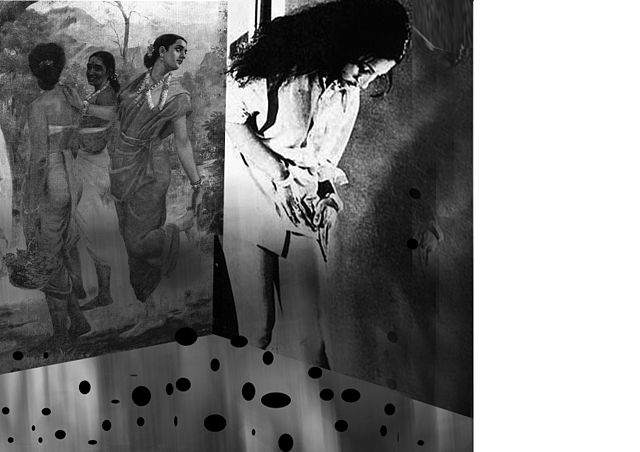
\includegraphics[width=\textwidth,height=8cm]{Kulasthree_Chapter_four_pic01.jpg}
\end{center}
%\caption*{പുലയർ - കെ പി പത്മനാഭ മേനോൻ - വാള്യം 3, (1929), 1984}
\end{figure}

\paragraph{}പത്തൊമ്പതാം നൂറ്റാണ്ടിന്റെ അവസാനദശകങ്ങൾ മുതൽ സമുദായപരിഷ്കരണപ്രസ്ഥാനങ്ങൾ ശക്തിപ്രാപിച്ചതോടുകൂടി പരമ്പരാഗത ജാതിസമൂഹങ്ങളുടെ തിരോധാനം ആരംഭിച്ചുവെന്ന് നമുക്കറിയാം. പരമ്പരാഗത ലിംഗമൂല്യങ്ങൾ മനുഷ്യത്വത്തിനെതിരാണെന്ന വിമർശനമുന്നയിച്ച ഈ പ്രസ്ഥാനങ്ങൾ അവയ്ക്കു പകരം പുതിയ മൂല്യങ്ങളെ മുന്നോട്ടുവച്ചു. ഇന്നു നമുക്കു പരിചിതങ്ങളായ ആൺ-പെൺഭേദങ്ങളും ഇരട്ടസദാചാരവും രൂപംപ്രാപിച്ചത് ഈ കാലഘട്ടത്തിലാണ്. സ്ത്രീകൾക്കിടയിൽത്തന്നെ 'നല്ല' സ്ത്രീയെയും 'ചീത്ത' സ്ത്രീയെയും വേർതിരിക്കുന്ന മാനദണ്ഡങ്ങൾ ഇതിന്റെ ഭാഗമായിരുന്നു. സ്ത്രീകളെ കുടുംബത്തിനുള്ളിലും സമൂഹത്തിലും സക്രിയരാക്കിത്തീർക്കാനുള്ള പരിശ്രമങ്ങളിലൂടെത്തന്നെയാണ് സ്ത്രീകളെ രണ്ടാംതരക്കാരാക്കി ചുരുക്കിയ ഈ മൂല്യങ്ങൾ വളർന്നുവികസിച്ചത്.

\section{നവവരേണ്യതയുടെ ലിംഗമൂല്യങ്ങൾ}
\label{ch4sec1}
\paragraph{}
കേരളത്തിൽ സ്ത്രീകളെ വിശേഷിപ്പിക്കാൻ ഉപയോഗിക്കുന്ന രണ്ടു പ്രയോഗങ്ങളാണിവ - 'തറവാട്ടിൽ പിറന്നവൾ', 'ചന്തപ്പെണ്ണ്'. 'മാന്യതയുള്ള സ്ത്രീ'യെ 'തറവാട്ടിൽ പിറന്നവൾ' എന്നു വിശേഷിപ്പിക്കുമ്പോൾ 'മാന്യതയില്ലാത്ത സ്ത്രീ'യെ 'ചന്തപ്പെണ്ണ്' എന്നു വിളിക്കുന്നു. ഈ വിളിയിൽ പഴയ ജാതിവ്യവസ്ഥയുടെ അംശങ്ങൾ പതിയിരിക്കുന്നുണ്ടെന്നു തീർച്ച. 'തറവാട്' എന്നാൽ പഴയ ജാത്യാഭിമാനത്തിന്റെ കേന്ദ്രമായിരുന്നല്ലോ. 'ചന്ത'യോ? പല ജാതിക്കാർ, പ്രത്യേകിച്ചു കീഴ്ജാതിക്കാർ, പല മതക്കാർ, ആണും പെണ്ണും ഒത്തുചേരുന്ന, 'ജാതിശുദ്ധം' തീരെ പാലിക്കാൻ പറ്റാത്ത ഇടമാണ്! അപ്പോൾ തറവാട്ടിലിരിക്കുന്നവൾ പരിശുദ്ധയും ചന്തയിൽ പണിയെടുക്കുന്നവൾ അശുദ്ധയുമായി കണക്കാക്കപ്പെട്ടത് സ്വാഭാവികം മാത്രം! പക്ഷേ, പരമ്പരാഗതമൂല്യവ്യവസ്ഥയ്ക്ക് 20-ാം നൂറ്റാണ്ടിൽ വൃദ്ധിയല്ല, ക്ഷയമാണ് സംഭവിച്ചതെന്ന് നമുക്കറിയാം. സമൂഹത്തിന്റെ മേൽത്തട്ടിലേക്ക് ഉയർന്നുവരാൻ വ്യക്തികളുടെ മുന്നിൽ നിരവധി വഴികൾ തുറന്നുകിട്ടിയ കാലമായിരുന്നു ഇത് - തറവാടിന്റെ മേൽവിലാസത്തിനുപുറമെ ഉന്നതവിദ്യാഭ്യാസം, ഉയർന്ന സാമ്പത്തികസ്ഥിതി, ഉദ്യോഗപദവി മുതലായവ സാമൂഹ്യമായ കയറ്റം നേടാനുള്ള മാർഗ്ഗങ്ങളായി ഇക്കാലത്തുയർന്നുവന്നു. നമ്മുടെ ഭാഷയിൽ, പക്ഷേ, ഇന്നും ഇത്തരം പ്രയോഗങ്ങൾ നിലനിൽക്കുന്നു. ജാതിപാരമ്പര്യത്തിന്റെ അവശിഷ്ടം മാത്രമാണോ ഇത്? പഴയ ജാതിസമുദായത്തിലെ പ്രമാണികൾക്കു പകരം 19-ാം നൂറ്റാണ്ടിലെ പുതിയ സാദ്ധ്യതകൾ പ്രയോജനപ്പെടുത്തിയ കൂട്ടരിൽനിന്നുണ്ടായ വർഗ്ഗം - 'നവവരേണ്യർ' എന്ന് നമുക്കവരെ വിളിക്കാം - പഴയ മൂല്യങ്ങളിൽ പലതിനേയും തള്ളിക്കളഞ്ഞു; പല പുതിയ മൂല്യങ്ങളെയും പരിപോഷിപ്പിച്ചു. എന്നാൽ, പഴയ വരേണ്യതയെ ഒന്നടങ്കം ഉപേക്ഷിച്ചുകൊണ്ടല്ല നവവരേണ്യർ തങ്ങളുടെ പുതിയ മൂല്യവ്യവസ്ഥയ്ക്കു രൂപംകൊടുത്തത്. പുതിയ മൂല്യങ്ങൾ സ്വീകരിക്കുന്നതിനുപുറമെ പഴയ വരേണ്യമൂല്യങ്ങളിൽനിന്ന് ചിലതുമാത്രം തെരഞ്ഞെടുത്ത് പരിഷ്ക്കരിച്ചുകൊണ്ടുകൂടിയാണ് നവവരേണ്യർ തങ്ങളുടെ മൂല്യവ്യവസ്ഥ ഉണ്ടാക്കിയത്.

\paragraph{}ആരായിരുന്നു, ഈ 'നവവരേണ്യർ'? 19-ാം നൂറ്റാണ്ടിലെ കേരളത്തിൽ, വിശേഷിച്ചും തിരുവിതാംകൂർ-കൊച്ചി പ്രദേശങ്ങളിൽ, നിരവധി കാതലായ സാമൂഹ്യസാമ്പത്തികമാറ്റങ്ങളുണ്ടായി. ബ്രിട്ടിഷ് അധികാരം നിലവിൽവന്നതോടെ ഈ രാജ്യങ്ങളിലെ ഭരണസംവിധാനങ്ങളെ നവീകരിക്കാനുള്ള ശ്രമമാരംഭിച്ചു. മിഷണറിമാരും പിൽക്കാലത്ത് സർക്കാരുകളും പ്രചരിപ്പിച്ച നവീനവിദ്യാഭ്യാസത്തിലൂടെ സർക്കാർ ഉദ്യോഗങ്ങളും പദവികളും നേടാമെന്നുവന്നു. പുതിയ വിദ്യാലയങ്ങളും കലാലയങ്ങളും സ്ഥാപിക്കപ്പെട്ടുതുടങ്ങി - അവിടങ്ങളിലും ഇംഗ്ലിഷ്‌വിദ്യാഭ്യാസം നേടിയവർക്കു ജോലിസാദ്ധ്യത തെളിഞ്ഞു. വ്യാപരരംഗം സജീവമായതോടുകൂടി അഭ്യസ്തവിദ്യർക്ക് അവിടെയും തൊഴിലവസരങ്ങൾ വർദ്ധിച്ചു. വ്യാപാരപ്രമുഖർ, വ്യവസായികൾ, അദ്ധ്യാപകർ, സർക്കാർ ഉദ്യോഗസ്ഥർ തുടങ്ങിയ കൂട്ടരടങ്ങിയ ഈ പുതിയ ജനവിഭാഗം 19-ാം നൂറ്റാണ്ടിന്റെ അവസാനദശകങ്ങളിൽ തിരുവിതാംകൂറിലും കൊച്ചിയിലും മലബാറിലും സജീവസാന്നിദ്ധ്യമായി. ആധുനിക പൊതുമണ്ഡലം ഇവരിലൂടെയാണ് രൂപപ്പെട്ടത് - അതായത് പത്രമാസികകൾ, ചർച്ചാവേദികൾ, വായനാസംഘങ്ങൾ മുതലായവ കൂടിച്ചേരുന്ന, സമൂഹത്തിന്റെ പൊതുപ്രശ്നങ്ങൾ ചർച്ചചെയ്യപ്പെടുന്ന, പുതിയ ഒരിടം ഇവരുടെ പ്രവർത്തനങ്ങളിലൂടെ രൂപപ്പെട്ടുതുടങ്ങി. അതുപോലെ, സ്വന്തം സമുദായങ്ങളെ കാലത്തിനൊത്ത് പരിഷ്ക്കരിക്കേണ്ടതെങ്ങനെ എന്ന ചോദ്യം ആദ്യമുന്നയിച്ചത് ആ സമുദായങ്ങളിലെ നവവരേണ്യർതന്നെ. മലബാറിലെ നായന്മാരിൽനിന്ന് സി. ശങ്കരൻനായർ, മാപ്പിളസമുദായത്തിൽനിന്ന് സനാ ഉല്ലാഹ് മക്തി തങ്ങൾ, തീയ്യ സമുദായത്തിൽനിന്ന് മൂർക്കോത്തു കുമാരൻ, കൊച്ചിയിലെ അരയസമുദായത്തിൽനിന്ന് പണ്ഡിറ്റ് കറുപ്പൻ, തിരുവിതാംകൂറിലെ ഈഴവരിൽനിന്ന് ഡോ.പൽപു, സുറിയാനി ക്രിസ്ത്യാനികൾക്കിടയിൽനിന്ന് പി.കെ. കൊച്ചീപ്പൻ തരകൻ തുടങ്ങിയ ആദ്യകാല സമുദായപരിഷ്ക്കർത്താക്കളും വക്താക്കളുമായിരുന്നവരെല്ലാം നവവരേണ്യരായിരുന്നു. ഇവരിൽ നല്ലൊരുവിഭാഗം പരമ്പരാഗത ജാതിവ്യവസ്ഥയിൽ മുന്തിയ സ്ഥാനമുണ്ടായിരുന്ന ജാതികളിൽ - അതായത്, നായർ - സുറിയാനി ക്രിസ്ത്യാനി ജാതികളിൽ - ഉൾപ്പെട്ടവരായിരുന്നു. ഇവരെക്കൂടാതെ തൊട്ടുകൂടാത്തവരായി ഗണിച്ചിരുന്ന ഈഴവ-തീയ്യ വിഭാഗങ്ങളിൽനിന്നും നവവരേണ്യരുണ്ടായിത്തുടങ്ങി. അതേസമയം പരമ്പരാഗതജാതിക്രമത്തിൽ മദ്ധ്യജാതികളിൽപ്പെട്ടിരുന്ന അരയസമുദായത്തിൽനിന്നും അധികംപേർ നവവരേണ്യവിഭാഗത്തിലേക്കു കടന്നില്ല. ഇരുപതാം നൂറ്റാണ്ടിൽ കേരളത്തിലുണ്ടായ സാമൂഹ്യ - രാഷ്ട്രീയ മാറ്റങ്ങളിൽനിന്നുള്ള നേട്ടങ്ങളധികവും കൊയ്തത് ഈ നവവരേണ്യവിഭാഗമായിരുന്നു.

\paragraph{}പൊതുവെ, മുതലാളിത്തവ്യവസ്ഥയുടെ സ്വത്തുനിയമങ്ങളോടുള്ള (അതായത് സ്വകാര്യസ്വത്തുടമസ്ഥതയ്ക്ക് അനുകൂലമായ നിയമങ്ങളോടുള്ള) കൂറ്, വ്യക്തികളുടെ സാമ്പത്തികവളർച്ചയിലൂടെയാണ് സമൂഹം പുരോഗമിക്കുന്നതെന്ന വിശ്വാസം, വ്യക്തികൾക്ക് മത്സരബുദ്ധിയോടെയുള്ള സാമ്പത്തികപ്രവർത്തനം നടത്താനുള്ള സാഹചര്യം ഒരുക്കലാണ് സമുദായപരിഷ്ക്കരണത്തിന്റെ ലക്ഷ്യമെന്ന വിശ്വാസം - ഇവ ഏറിയോ കുറഞ്ഞോ നവവരേണ്യമൂല്യവ്യവസ്ഥയിൽ ഉൾപ്പെട്ടിരുന്നു. ഈ മൂല്യങ്ങളെല്ലാംതന്നെ പാശ്ചാത്യലോകത്തുനിന്ന് ഇങ്ങോട്ടു പ്രവഹിച്ചവയായിരുന്നു. എന്നാൽ ഇവയോടൊപ്പം മറ്റുപല ആശയങ്ങളും പാശ്ചാത്യരാജ്യങ്ങളിൽനിന്ന് ഇവിടേക്കെത്തിയിരുന്നു. മനുഷ്യർ തമ്മിലുള്ള അടിസ്ഥാനപരമായ തുല്യത, സമത്വം, സാഹോദര്യം - ഈ ആശയങ്ങളും പാശ്ചാത്യലോകത്തുനിന്ന് ഇവിടെ എത്തിയവയാണ്. ഇവയ്ക്ക്, പക്ഷേ, ഭാഗികമായ അംഗീകാരമേ നവവരേണ്യർ നൽകിയുള്ളൂ. അഥവാ, നവവരേണ്യരുടെ താൽപര്യങ്ങൾക്ക് കോട്ടംതട്ടാത്തവിധത്തിൽമാത്രമേ അവ പ്രയോഗിക്കപ്പെട്ടുള്ളൂ. ശ്രീനാരായണഗുരുവിനെപ്പോലുള്ളവരുടെ സമത്വചിന്തയെപ്പോലും ഇത്തരത്തിൽ ന്യൂനീകരിക്കാൻ നവവരേണ്യർക്കു കഴിഞ്ഞു.

\paragraph{}
അതുകൊണ്ടുതന്നെ പാശ്ചാത്യലോകത്ത് വിമോചനകരങ്ങളായി വ്യാഖ്യാനിക്കപ്പെട്ട പല ആശയങ്ങളും ഇവിടെ തീരെ ചർച്ചചെയ്യപ്പെട്ടില്ല; അല്ലെങ്കിൽ ന്യൂനീകരിക്കപ്പെട്ടു. എന്തായാലും നവവരേണ്യർക്ക് അനുകൂലമായ വിധത്തിൽ പാശ്ചാത്യ ആശയങ്ങളെയും പ്രയോഗങ്ങളെയും എങ്ങനെ മാറ്റിത്തീർക്കാമെന്ന വിചാരം 20-ാം നൂറ്റാണ്ടിലെ ചർച്ചകളിൽ വ്യക്തമായും കാണാനുണ്ട്. ഉദാഹരണത്തിന്, 1930കൾമുതൽ ഇവിടെയാരംഭിച്ച ജനനനിയന്ത്രണചർച്ച തന്നെയെടുക്കാം. ഇതിൽ നവവരേണ്യർക്കിടയിലെ യാഥാസ്ഥിതികർ ഉന്നയിച്ച സംശയങ്ങൾ മൂന്നായിരുന്നു: ഒന്ന്, ജനനനിയന്ത്രണം വ്യാപകമായാൽ 'അറിവില്ലാത്ത' ജനങ്ങൾക്കിടയിൽ ലൈംഗിക അരാജകത്വം വ്യാപിക്കില്ലേ? രണ്ട്, സ്ത്രീകൾക്ക് അച്ചടക്കവും അനുസരണയും ഇല്ലാതാകില്ലേ? മാത്രമല്ല, ജനനനിയന്ത്രണം സമൂഹത്തിന്റെ മേൽത്തട്ടിൽ വ്യാപകമായാൽ 'താണതരക്കാർ' പെറ്റുപെരുകുകയില്ലേ? ഇതായിരുന്നു മൂന്നാമത്തെ ഭയം. ജനനനിയന്ത്രണത്തെ അനുകൂലിച്ച നവവരേണ്യരോ? അവർക്കും പേടി 'താണതരക്കാരെ' ആയിരുന്നു. ജനനനിയന്ത്രണം വ്യാപിപ്പിച്ചാൽ 'താണതരക്കാരു'ടെ എണ്ണം കുറയ്ക്കാനൊക്കുമെന്നായിരുന്നു അവരുടെ വിശ്വാസം! ചുരുക്കിപ്പറഞ്ഞാൽ, അനുകൂലിച്ചാലും പ്രതികൂലിച്ചാലും ജനനനിയന്ത്രണത്തിൽ നവവരേണ്യരുടെ താൽപര്യങ്ങളെക്കുറിച്ചായിരുന്നു ചർച്ച.

\paragraph{}പുതിയ ലിംഗമൂല്യങ്ങളുടെ കാര്യത്തിലും പൂർണ്ണമായ സ്ത്രീപുരുഷതുല്യത നവവരേണ്യർക്ക് ആകർഷകമായി തോന്നിയിരുന്നില്ല. സ്ത്രീയുടെ 'വ്യത്യസ്തത'യെ അതായത്, പുരുഷനിൽനിന്ന് വ്യത്യസ്തമായി സ്ത്രീക്ക് പ്രസവം, ബാലപരിചരണം എന്നീ രണ്ടു ധർമ്മങ്ങളുണ്ടെന്നതിന് ഊന്നൽ നൽകിക്കൊണ്ടാണ് നവവരേണ്യലിംഗമൂല്യങ്ങൾ ശക്തമായത്. 'തുല്യത' എന്നാൽ ആണിനേയും പെണ്ണിനേയും ഒരേ അച്ചിലിട്ട് വാർക്കലാണെന്ന തെറ്റായ വ്യാഖ്യാനത്തിന് ഏറെ പ്രചാരം ലഭിക്കുകയും ചെയ്തു. 1930കളായപ്പോഴേക്കും ഈ ദുർവ്യാഖ്യാനത്തെ ചോദ്യംചെയ്ത ചില സ്ത്രീശബ്ദങ്ങൾ കേട്ടുതുടങ്ങിയിരുന്നു. 1938ൽ കോച്ചാട്ടിൽ കല്യാണിക്കുട്ടിയമ്മ (മിസിസ്സ്. സി. കുട്ടൻനായർ) ഇതിനെ വിമർശിച്ചുകൊണ്ട് ഇങ്ങനെ എഴുതി:

\begin{quotation}
\noindent സമത്വം ഞങ്ങളുടെ ഇന്നത്തെ പലേ ദുരിതങ്ങളേയും നീക്കംചെയ്യുമെന്നു സ്ത്രീകളായ ഞങ്ങളിൽ പലരും ബലമായി വിശ്വസിക്കുന്നു. എല്ലാവരേയും ഒരേ അച്ചിലിട്ടു വാർക്കാനല്ല സമത്വവാദിനികൾ ഉദ്ദേശിക്കുന്നത്. നേരെമറിച്ച്, സമത്വംകൊണ്ടേ വ്യക്തിപരമായ വളർച്ച സാദ്ധ്യമാകൂ. നമുക്കു നമ്മുടെ സ്വഭാവവിശേഷങ്ങളെപ്പറ്റി ഇന്നും എത്രയും അപൂർണ്ണമായ ജ്ഞാനമേ ഉള്ളൂ. 'പുരുഷത്വം', 'സ്ത്രീത്വം' എന്നീ അവ്യക്തവചനങ്ങൾകൊണ്ടു നാം യഥാർത്ഥത്തിൽ സൂചിപ്പിക്കുന്നതെന്ത്? മനഃശാസ്ത്രഗവേഷണങ്ങൾ, ലിംഗപരമായ സംഗതിയെക്കുറിച്ച് നമുക്കുള്ള അജ്ഞതയെ വെളിവാക്കുന്നില്ലേ? നമ്മുടെ അപൂർണ്ണജ്ഞാനത്തിന്റെ സന്താനങ്ങളായ സദാചാരനിബന്ധനകൾ എത്ര വ്യക്തികളുടെ വളർച്ചയെ തടയുന്നു!
\flushright{(മിസിസ്സ് സി. കുട്ടൻ നായർ,
'സ്ത്രീപുരുഷസമത്വത്തിനുള്ള ചില പ്രതിബന്ധങ്ങൾ', മാതൃഭൂമി വിശേഷാൽപ്രതി, 1938)}

\end{quotation}


\paragraph{}പക്ഷേ, ഇതൊക്കെ കേവലം ഒറ്റപ്പെട്ട ശബ്ദങ്ങളായിരുന്നു. ലിംഗവ്യത്യാസത്തെ അടിസ്ഥാനപ്പെടുത്തിയ ഒരു പുതിയ സമുദായമാന്യത അപ്പോഴേക്കും രൂപമെടുത്തുകഴിഞ്ഞിരുന്നു. സ്ത്രീയുടെ സ്ഥാനം ഗൃഹത്തിനുള്ളിലാണെന്നും, ഭർത്താവിലൂടെയാണ് അവളുടെ സാമൂഹിക അംഗത്വമെന്നുമുള്ള ധാരണകൾ ഇവിടത്തെ സമുദായപരിഷ്ക്കരണപ്രസ്ഥാനങ്ങളിൽ രൂഢമൂലമായിക്കഴിഞ്ഞിരുന്നു.


\section{'ഉത്തമസ്ത്രീ' പിറക്കുന്നു}
\label{ch4sec2}
\paragraph{}19-ാം നൂറ്റാണ്ടിൽ പല കാരണങ്ങളാൽ കേരളത്തിലെ പരമ്പരാഗതജാതിവ്യവസ്ഥയുടെ അടിത്തറ ഇളകാൻ തുടങ്ങി. ബ്രിട്ടിഷുകാരുടെ മേൽക്കോയ്മ ഇവിടത്തെ പരമ്പരാഗതരാജവംശങ്ങളുടെയും പരമാധികാരത്തെ ഇല്ലാതാക്കി - ജാതിമാമൂലിന്റെ സംരക്ഷകർ ഇവരായിരുന്നല്ലോ. മിഷണറിമാരുടെ വരവ് കീഴ്ജാതികൾക്കു താങ്ങായി. അവരുടെമേൽ അടിച്ചേൽപ്പിക്കപ്പെട്ടിരുന്ന പല നികുതികളും, കൂലിയില്ലാത്ത അദ്ധ്വാനവും നിറുത്തൽ ചെയ്യിക്കുന്നതിൽ മിഷണറിമാർ വലിയ പങ്കുവഹിച്ചു. ആധുനികവിദ്യാഭ്യാസം മിഷണറിപള്ളിക്കൂടങ്ങളിലൂടെ വ്യാപകമായതോടെ കീഴ്ജാതിക്കാരിൽ ചിലകൂട്ടർക്ക് പുതിയ അവസരങ്ങൾ ലഭിച്ചുതുടങ്ങി. കച്ചവടവും കുടിയേറ്റസാദ്ധ്യതയും വർദ്ധിച്ചതോടുകൂടി അവരിൽ ചിലർ സാമ്പത്തിക നേട്ടങ്ങളും കൈവരിച്ചു. 'മാറുമറയ്ക്കൽസമരം' പോലുള്ള നിർണ്ണായകപോരാട്ടങ്ങളിലൂടെ മേൽജാതിക്കാരുടെ അധികാരങ്ങൾ നിയന്ത്രിക്കപ്പെട്ടു. (കാണുക \ref{ch7sec2}) 1865ലെ വിളംബരപ്രകാരം തിരുവിതാംകൂർ സർക്കാർ കുടിയാന്മാർക്ക് ഭൂമിയിൽ ഉടമസ്ഥാവകാശം ലഭിച്ചു. ഇതേകാലത്തുതന്നെ പരമ്പരാഗത മേലാളസമുദായങ്ങളും മാറ്റത്തിനു വിധേയമായി. വികസിച്ചുവന്ന കച്ചവടരംഗവും വിപണിയും വാണിജ്യകൃഷിയും സുറിയാനിക്രിസ്ത്യാനിസമുദായത്തിന് വർദ്ധിച്ച അവസരങ്ങൾ നൽകി. പുതിയ വിദ്യാഭ്യാസത്തിലൂടെ അവർ ഈ രംഗങ്ങളിൽ കുതിച്ചുയർന്നു. നായർതറവാടുകളുടെ ജാത്യാധികാരം അൽപ്പം ക്ഷയിച്ചെങ്കിലും പുതിയ വിദ്യാഭ്യാസത്തിലൂടെ ഭരണരംഗത്തും സാംസ്കാരികരംഗത്തും അവർ പിടിച്ചുനിന്നു. നമ്പൂതിരിമാർ മാത്രമാണ് ഈ പുതിയ അന്തരീക്ഷത്തോട് ഇണങ്ങിച്ചേരാൻ വിസമ്മതം കാട്ടിയത്. ഇവരും ഇരുപതാം നൂറ്റാണ്ടിൽ നിലപാടു മാറ്റി..

\paragraph{}പൊതുവെ ജാതിവ്യവസ്ഥയ്ക്കെതിരെ രൂക്ഷവിമർശനം ഉയർന്നുവന്ന കാലമായിരുന്നു 19-ാം നൂറ്റാണ്ടിന്റെ അവസാനദശകങ്ങൾ. ദൈവദൃഷ്ടിയിൽ തുല്യരായ, ദൈവം ഒരുപോലെ സൃഷ്ടിച്ച, മനുഷ്യരെ പരസ്പരം വേർതിരിക്കുന്ന ഈ വ്യവസ്ഥ പ്രകൃതിക്കും മനുഷ്യനും ദൈവത്തിനും ഒരുപോലെ എതിരാണെന്ന് മിഷണറിമാരും സഹചാരികളും വാദിച്ചു. മിഷണറിസ്വാധീനത്തിനു പുറത്തുനിന്നുകൊണ്ട് പാശ്ചാത്യരാഷ്ട്രീയചിന്തയിൽനിന്ന് സമത്വവാദങ്ങൾ കടമെടുത്തുകൊണ്ട് എഴുതിയ ചിലരുമുണ്ടായിരുന്നു. ഈ രണ്ടുകൂട്ടരും യോജിച്ച ഒരു കാര്യമുണ്ടായിരുന്നു - സ്ത്രീപുരുഷന്മാർ തമ്മിലുള്ള വ്യത്യാസത്തെ അവരുടെ ശാരീരികമായ പ്രത്യേകതകൾകൊണ്ട് വിശദീകരിക്കാമെന്ന അവകാശവാദം. സ്ത്രീയുടെയും പുരുഷന്റെയും ശാരീരികപ്രത്യേകതകൾക്കിണങ്ങുന്ന സ്വഭാവഗുണങ്ങളും മനോഗതിയും പ്രകൃതിതന്നെ അവർക്കു നൽകിയിരിക്കുന്നുവെന്നും ഇവയിലൂടെയാണ് സ്ത്രീയുടെയും പുരുഷന്റെയും സാമൂഹികനില നിർണ്ണയിക്കേണ്ടതുമെന്നും മിഷണറിമാരും മറ്റു പരിഷ്ക്കരണകുതുകികളും ഒരുപോലെ വാദിച്ചു. ഇതുപ്രകാരം സ്ത്രീയുടെ ശരിയായ ഇടം ഗൃഹമാണെന്നു കൽപ്പിക്കപ്പെട്ടു. വീട്ടുജോലി, പ്രസവിക്കൽ, കുട്ടികളെ വളർത്തൽ തുടങ്ങിയ കർമ്മങ്ങളും പൊതുവെ വികാരങ്ങളിലൂടെ കുടുംബാംഗങ്ങളെ സ്വാധീനിച്ച് നല്ലവഴിക്കു നടത്താനുള്ള ഉത്തരവാദിത്വവും സ്ത്രീക്കുള്ളതാണെന്നും വന്നു. പുറംലോകത്തിൽനിന്നു വ്യത്യസ്തമായി മദമത്സരമില്ലാത്ത, സമാധാനവും സ്നേഹവും നിലനിൽക്കേണ്ട ഇടമാണ് ഗൃഹമെന്നും അതിനു തക്കതായ മനോഗുണങ്ങൾ ഓരോ സ്ത്രീയിലും പ്രകൃതിതന്നെ നിക്ഷേപിച്ചിട്ടുണ്ടെന്നുമാണ് നവവരേണ്യലേഖകരും മിഷണറിമാരും വാദിച്ചത്. സ്നേഹം, ദയ, ക്ഷമ, വാത്സല്യം, വാക്കുകളിലൂടെയും കണ്ണീരിലൂടെയും അഭ്യർത്ഥനയിലൂടെയും മറ്റു മനുഷ്യരെ സ്വാധീനിക്കാനുള്ള ശക്തി - ഇതൊക്കെ സ്ത്രീക്ക് സഹജമായിത്തന്നെ ലഭിക്കുന്നുണ്ടത്രെ. എന്നാൽ പരമ്പരാഗതകുടുംബരീതികൾ ഈവക ഗുണങ്ങളെ തീരെ പോഷിപ്പിക്കുന്നില്ലെന്നും, അതുകൊണ്ടുതന്നെ പരമ്പരാഗതകുടുംബങ്ങളിലെ സ്ത്രീകളുടെ യഥാർത്ഥ 'സ്ത്രീഗുണം' വെറുതെ പാഴാവുകയാണെന്നും ഇക്കൂട്ടർ പരിതപിച്ചു. സ്ത്രീയുടെ 'സവിശേഷഗുണങ്ങ'ളെ പരിപോഷിപ്പിക്കാനുതകുന്നതരം വിദ്യാഭ്യാസം അവർക്കു നൽകുക; കുടുംബരീതികളിൽ മാറ്റം വരുത്തുക; വിവാഹസമ്പ്രദായങ്ങൾ പരിഷ്ക്കരിക്കുക - സ്ത്രീകളുടെ 'യഥാർത്ഥ സ്ത്രീത്വ'ത്തെ വീണ്ടെടുക്കാൻവേണ്ടി 19-ാം നൂറ്റാണ്ടിന്റെ അവസാനകാലത്തും 20-ാം നൂറ്റാണ്ടിന്റെ ആദ്യദശകങ്ങളിലും പല ലേഖകരും മുന്നോട്ടുവച്ച നിർദ്ദേശങ്ങളാണിവ.
\paragraph{}

അപ്പോൾ, ജാതിവ്യവസ്ഥ പൂർണ്ണമായും ഉന്മൂലനംചെയ്യപ്പെട്ട സമൂഹത്തെ വിഭാവനം ചെയ്യുമ്പോഴും സ്ത്രീപുരുഷവ്യത്യാസം അതിനുള്ളിൽ നിലനിന്നിരുന്നുവെന്നർത്ഥം. സ്ത്രീപുരുഷന്മാർ തമ്മിലുള്ള വ്യത്യസ്തത അവർ തമ്മിലുള്ള തുല്യതയ്ക്കു വിഘാതമാവില്ലെന്ന ധാരണ ഇതിൽ അന്തർലീനമായിരുന്നു. വീടിനും പുറംലോകത്തിനും ഒരേ അധികാരവും അംഗീകാരവും ലഭിക്കുന്ന സമൂഹങ്ങളിൽ സ്ത്രീപുരുഷതുല്യത സ്വാഭാവികമായും ഉണ്ടാകുമെന്ന ശുഭാപ്തിവിശ്വാസം തുളുമ്പിനിൽക്കുന്നതും കാണാം.

\captionof{mybox}{മലയാളിസ്ത്രീകളുടെ തൊഴിൽപങ്കാളിത്തം}\label{ch3box2} % place the caption
\begin{tcolorbox}[%
 breakable, % make the box breakable
  arc=0mm, 
  left=1pt, right = 1pt, 
  boxrule=0mm,
  colback = {blue!10}, % since shadow-gray was not defined
] 
ഇരുപതാംനൂറ്റാണ്ടിൽ മലയാളിസ്ത്രീകളുടെ തൊഴിൽപങ്കാളിത്തനിരക്കിൽ ഗണ്യമായ ഇടിവുണ്ടായിട്ടുണ്ടെന്ന് സാമൂഹ്യശാസ്ത്രജ്ഞർ ചൂണ്ടിക്കാണിക്കുന്നു. 1901 മുതൽ 2011വരെയുള്ള കണക്കുകളാണ് താഴെ. പുരുഷന്മാരും സ്ത്രീകളും തമ്മിലുള്ള വിടവും വർദ്ധിച്ചുവെന്നു കാണാം. 

\begin{tabular}{ l c c r }
വർഷം &	പുരുഷൻ	& സ്ത്രീ &	വിടവ് \\
\hline
1901 &	56.3	&  32.7&	23.6\\
1911	& 53.8	& 28.9	& 24.9\\
1921&	51.1&	24.5&	26.6\\
1931	&50.0&	35.9&	14.1\\
1941&	ലഭ്യമല്ല&	ലഭ്യമല്ല	&ലഭ്യമല്ല\\
1951&	46.7&	18.3	&28.4\\
1961	&47.2	&19.7&	27.5\\
1971&	45.2	&14.6&	30.6\\
1981&	44.9&	16.6&	28.3\\
1991&	47.6&	15.9&	31.7\\
2001&	50.4	&15.3&	35.7\\
\end{tabular}

(S. Irudaya Rajan, Sreerupa, "Gender Disparity in Kerala : A Critical Reinterpretation', Swapna Mukhopadhyay (ed), The Enigma of the Kerala Woman, New Delhi, 2007, പുറം. 46)
\\
1931ൽ സ്ത്രീകൾ കൂടുതലായി തൊഴിൽരംഗത്തു പ്രവേശിച്ചതായി കാണുന്നുവെങ്കിലും 1951ൽ അവരുടെ തൊഴിൽപങ്കാളിത്തനിരക്ക് തീരെ കുറഞ്ഞതായി കാണുന്നു. പിന്നീട് ഏറെക്കുറെ താഴേക്കുതന്നെയാണാ അതിന്റെ പോക്ക്. എന്നാൽ 1931ലെ വർദ്ധനവ് സെൻസസ് വിവരശേഖരണരീതിയിൽ ആ തവണ ഉണ്ടായ മാറ്റംകൊണ്ടാകാം.
\end{tcolorbox}

\paragraph{}ജോസഫ് മൂളിയിൽ രചിച്ച സുകുമാരി (1897) എന്ന നോവലിൽ ജാതിവ്യത്യാസത്തെയും അസമത്വത്തെയും ന്യായീകരിച്ച ജാതിക്രമവും ആൺ-പെൺ വ്യത്യാസത്തിലൂന്നിയ ലിംഗക്രമവും തമ്മിൽ നേർക്കുനേർ ഇടയുന്ന ഒരു സന്ദർഭമുണ്ട്. കീഴ്ജാതിയിൽനിന്ന് ക്രിസ്തുമതം സ്വീകരിച്ച ഒരുവനാണ് ലിംഗക്രമത്തിന്റെ വക്താവായി നോവലിൽ പ്രത്യക്ഷപ്പെടുന്നത്. ഇതു കീഴ്ജാതികൾക്ക് നൽകിയ ആത്മവിശ്വാസം ശ്രദ്ധേയമാണ്.
